\documentclass[../main.tex]{subfiles}

\begin{document}

\ifSubfilesClassLoaded{

    %\tableofcontents
    
 \setcounter{chapter}{10}
}{}

\chapter{ HW11 }
 代靖涵 25120222201319
\begin{exercise}{}{}
问题1 计算下列空间的基本群:
\begin{enumerate}
\item \(\mathbb{R}^2\) 去掉 \(3\) 个点.
\item \(S^2\) 去掉 \(3\) 个点.
\item \(T^2\) 去掉 \(3\) 个点.
\item \(\theta\)-空间.(示意图如下)
\end{enumerate}
\begin{center}
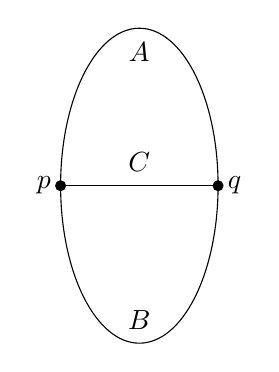
\begin{tikzpicture}
\draw (0,0) ellipse (1 and 2);
\draw (-1,0) -- (1,0);
\fill (-1,0) circle (2pt) node[left] {$p$};
\fill (1,0) circle (2pt) node[right] {$q$};
\node at (0,1.7) {$A$};
\node at (0,-1.7) {$B$};
\node at (0,0.3) {$C$};
\end{tikzpicture}
\end{center}
(描述形变收缩时画图示意即可, 无需写下具体的同伦映射)
\end{exercise}

\begin{proof}
    \begin{enumerate}
        \item \(  \mathbb{R} ^{2}  \)去掉三个点\(  p_1,p_2,p_3  \) , 不妨设这三个点在单位圆盘内, 则\(  \mathbb{R} ^{2}  \setminus \left\{ p_1,p_2,p_3 \right\}\) 可以形变收缩到 \(  D^{2}\setminus \left\{ p_1,p_2,p_3 \right\}  \). 然后再做如下形变收缩
        
    \begin{center}
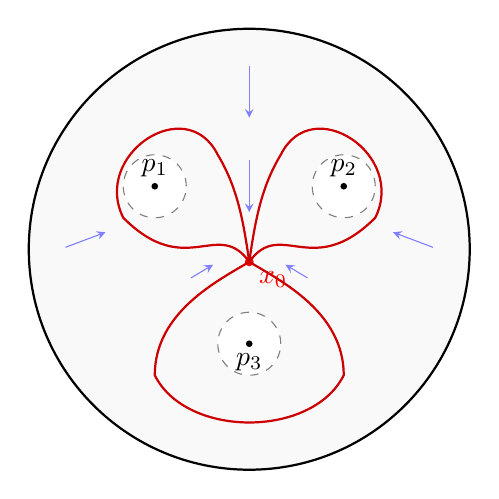
\begin{tikzpicture}[scale=0.8]
    % 定义样式
    \tikzstyle{point}=[circle, fill=black, inner sep=1.5pt]
    \tikzstyle{hole}=[circle, draw=gray, dashed, fill=white, inner sep=0pt, minimum size=0.8cm]
    \tikzstyle{skeleton}=[thick, red!80!black]
    \tikzstyle{arrowstyle}=[->, >=stealth, blue!50, shorten >=2pt, shorten <=2pt]

    % 1. 画大圆盘 (代表 R^2 收缩后的有界区域)
    \draw[thick, fill=gray!5] (0,0) circle (3.5cm);


    % 2. 画三个被挖去的点 (或者小孔洞)
    \node[hole] (h1) at (-1.5, 1) {};
    \node[hole] (h2) at (1.5, 1) {};
    \node[hole] (h3) at (0, -1.5) {};
    
    % 标记点的位置
    \fill (h1.center) circle (1.5pt) node[above] {$p_1$};
    \fill (h2.center) circle (1.5pt) node[above] {$p_2$};
    \fill (h3.center) circle (1.5pt) node[below] {$p_3$};

    % 3. 画骨架 (Wedge of circles 的嵌入形式)
    % 基点
    \coordinate (base) at (0, -0.2);
    \fill[red] (base) circle (2pt) node[below right, red] {$x_0$};

    % 回路 1 (绕 p1)
    \draw[skeleton] (base) .. controls (-0.5, 0.5) and (-1, -0.5) .. (-2, 0.5) 
                    .. controls (-2.5, 1.5) and (-1, 2.5) .. (-0.5, 1.5)
                    .. controls (-0.2, 1) and (-0.1, 0.5) .. (base);
    
    % 回路 2 (绕 p2)
    \draw[skeleton] (base) .. controls (0.5, 0.5) and (1, -0.5) .. (2, 0.5) 
                    .. controls (2.5, 1.5) and (1, 2.5) .. (0.5, 1.5)
                    .. controls (0.2, 1) and (0.1, 0.5) .. (base);

    % 回路 3 (绕 p3)
    \draw[skeleton] (base) .. controls (-0.5, -0.5) and (-1.5, -1) .. (-1.5, -2)
                    .. controls (-1, -3) and (1, -3) .. (1.5, -2)
                    .. controls (1.5, -1) and (0.5, -0.5) .. (base);

    % 4. 画形变收缩的流向箭头 (示意)
    % 从边界向内
    \draw[arrowstyle] (-3, 0) -- (-2.2, 0.3);
    \draw[arrowstyle] (3, 0) -- (2.2, 0.3);
    \draw[arrowstyle] (0, 3) -- (0, 2);
    
    % 从孔洞之间挤压向骨架
    \draw[arrowstyle] (0, 1.5) -- (0, 0.5); % p1 p2 之间
    \draw[arrowstyle] (-1, -0.5) -- (-0.5, -0.2); % p1 p3 之间
    \draw[arrowstyle] (1, -0.5) -- (0.5, -0.2); % p2 p3 之间

\end{tikzpicture}
\end{center}
\begin{center}
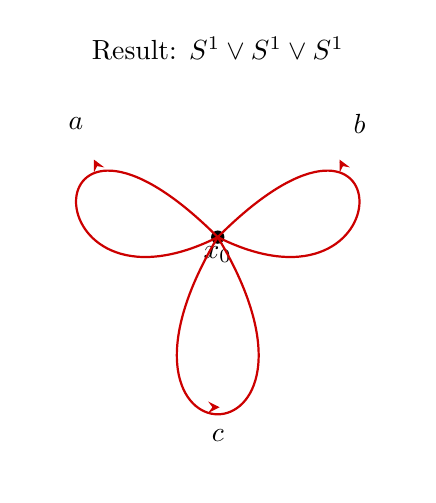
\begin{tikzpicture}[scale=1.2]
    % 定义样式
    \tikzstyle{loopstyle}=[thick, red!80!black, ->, >=stealth]

    % 基点
    \coordinate (O) at (0,0);
    \fill (O) circle (2pt) node[below] {$x_0$};

    % 这里的形状是为了好看，画成花瓣状
    
    % 左圈 (对应 p1)
    \draw[thick, red!80!black] (O) .. controls (-2, 2) and (-2, -1) .. (O);
    % 添加方向箭头和标签
    \draw[thick, red!80!black, ->, >=stealth] (-1.3, 0.8) -- (-1.31, 0.82); 
    \node at (-1.5, 1.2) {$a$};

    % 右圈 (对应 p2)
    \draw[thick, red!80!black] (O) .. controls (2, 2) and (2, -1) .. (O);
    % 添加方向箭头和标签
    \draw[thick, red!80!black, ->, >=stealth] (1.3, 0.8) -- (1.29, 0.82);
    \node at (1.5, 1.2) {$b$};

    % 下圈 (对应 p3)
    \draw[thick, red!80!black] (O) .. controls (-1.5, -2.5) and (1.5, -2.5) .. (O);
    % 添加方向箭头和标签
    \draw[thick, red!80!black, ->, >=stealth] (0, -1.8) -- (0.02, -1.8);
    \node at (0, -2.1) {$c$};

    \node at (0, 2) {Result: $S^1 \vee S^1 \vee S^1$};
\end{tikzpicture}

\end{center}

由Van kampen定理, 取 \(  x_0  \)的一个充分小的邻域 \(  U  \), 使得 \(  U  \)是可缩与 \(  x_0  \)的.  则 每个 \(  S_1\cup U  \)都形变收缩到\(  S^{1}  \), 自身, 由Van  Kampen 定理,  \[
 \pi _1 \left( \mathbb{R} ^{2}\setminus \left\{ p_1,p_2,p_2 \right\} \right)\simeq  \pi _1 \left( S^{1}\vee S^{1}\vee S^{1} \right)\simeq \mathbb{Z} *\mathbb{Z} *\mathbb{Z}   
\]

\item 去掉的三个点扩大成三个空腔, 原空间形变收缩到如下灯笼状空间

\begin{center}
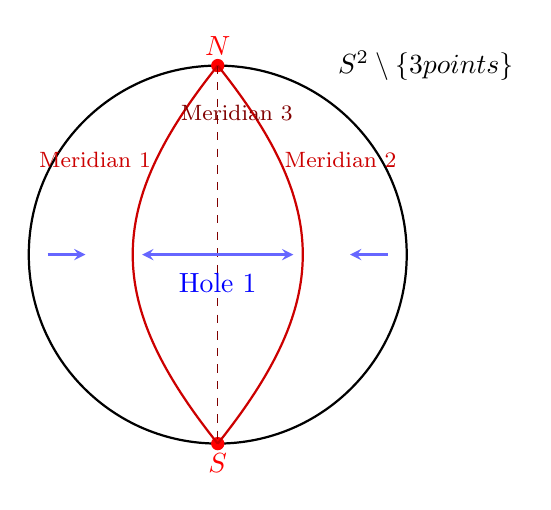
\begin{tikzpicture}[scale=1.2]
    % 定义样式
    \tikzstyle{meridian}=[thick, red!80!black]
    \tikzstyle{hidden}=[dashed, red!50!black]
    \tikzstyle{holearrow}=[->, >=stealth, blue!60, thick]

    % 1. 画球体轮廓
    \draw[thick] (0,0) circle (2cm);
    \node at (2.2, 2) {$S^2 \setminus \{3 \text{ points}\}$};

    % 定义南北极
    \coordinate (N) at (0, 2);
    \coordinate (S) at (0, -2);
    \fill[red] (N) circle (2pt) node[above] {$N$};
    \fill[red] (S) circle (2pt) node[below] {$S$};

    % 2. 画三条经线 (骨架)
    % 经线 1 (左前)
    \draw[meridian] (N) .. controls (-1.2, 0.5) and (-1.2, -0.5) .. (S);
    % 经线 2 (右前)
    \draw[meridian] (N) .. controls (1.2, 0.5) and (1.2, -0.5) .. (S);
    % 经线 3 (背面 - 稍微偏一点以便看到)
    \draw[hidden] (N) -- (S);

    % 3. 示意扩大的空腔 (Holes)
    % 左侧空腔中心
    \node at (-1.5, 0) (H1) {};
    % 右侧空腔中心
    \node at (1.5, 0) (H2) {};
    % 中间(正面)空腔中心
    \node at (0, 0) (H3) {};

    % 4. 画扩大的箭头
    % 中间空腔向两侧挤压
    \draw[holearrow] (0, 0) -- (0.8, 0);
    \draw[holearrow] (0, 0) -- (-0.8, 0);
    \node[blue] at (0, -0.3) {Hole 1};

    % 左侧空腔向内挤压
    \draw[holearrow] (-1.8, 0) -- (-1.4, 0);
    
    % 右侧空腔向内挤压
    \draw[holearrow] (1.8, 0) -- (1.4, 0);

    % 5. 标注经线
    \node[red!80!black, font=\footnotesize] at (-1.3, 1) {Meridian 1};
    \node[red!80!black, font=\footnotesize] at (1.3, 1) {Meridian 2};
    \node[red!50!black, font=\footnotesize] at (0.2, 1.5) {Meridian 3};

\end{tikzpicture}
\end{center}
将第三条经线收缩到一个点, 使得 \(  N,S  \)重合,  得到 \(  S^{1}\vee S^{1}  \). 同样地, 由Van  Kampen定理\[
 \pi _1 \left( S^{2}\setminus \left\{ p_1,p_2,p_3 \right\} \right)\simeq  \pi _1 \left( S^{1}\vee S^{1} \right)\simeq \mathbb{Z} *\mathbb{Z}   
\] \\ 
 

\item 
现在多边形的中心上挖去一个点\(  p_1  \) , 令多边形表示从\(p_1    \) 收缩到边界的\(  a,b  \)的边缘附近. 

\begin{center}
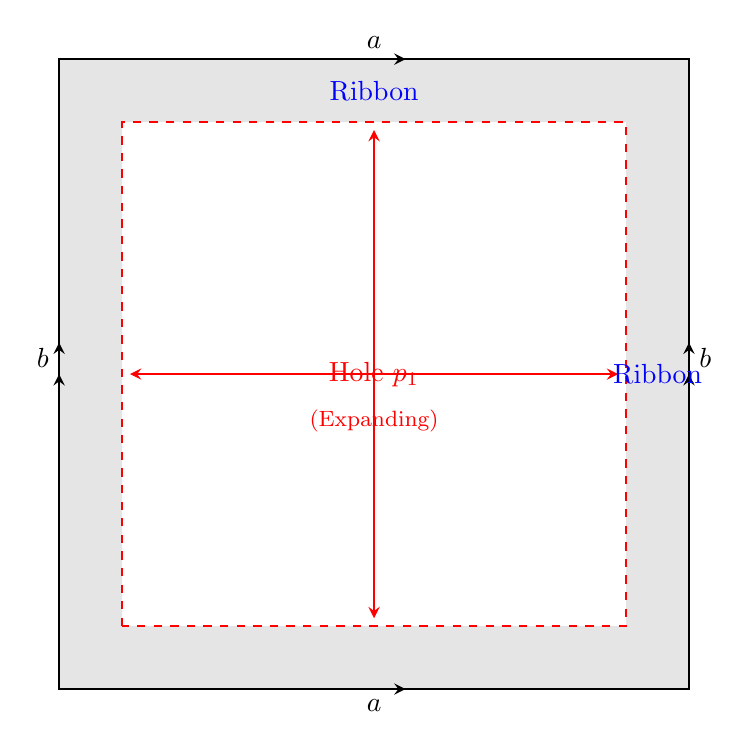
\begin{tikzpicture}[scale=2]
    % --- 样式设置 ---
    \tikzstyle{arrowstyle}=[->, >=stealth, thick, black]
    \tikzstyle{force}=[->, >=stealth, thick, red]

    % 1. 填充细纸带区域 (灰色)
    % 使用 even odd rule 挖空中间
    \fill[gray!20, even odd rule] (-2,-2) rectangle (2,2) (-1.6,-1.6) rectangle (1.6,1.6);

    % 2. 画外边界 (环面的基本域边界)
    \draw[thick] (-2,-2) rectangle (2,2);

    % 3. 画内边界 (洞的边缘, 正在扩张)
    \draw[thick, dashed, red] (-1.6,-1.6) rectangle (1.6,1.6);

    % 4. 标记粘合关系 (表明这是环面)
    % 上下边 (a)
    \draw[arrowstyle] (-0.2, 2) -- (0.2, 2) node[midway, above] {$a$};
    \draw[arrowstyle] (-0.2, -2) -- (0.2, -2) node[midway, below] {$a$};
    % 左右边 (b) - 使用双箭头区分
    \draw[arrowstyle] (-2, -0.2) -- (-2, 0) node[midway, left] {}; 
    \draw[arrowstyle] (-2, 0) -- (-2, 0.2) node[midway, left] {$b$};
    \draw[arrowstyle] (2, -0.2) -- (2, 0) node[midway, right] {};
    \draw[arrowstyle] (2, 0) -- (2, 0.2) node[midway, right] {$b$};

    % 5. 画挤压箭头 (表示洞在变大, 把空间挤成纸带)
    \draw[force] (0, 0) -- (0, 1.55);
    \draw[force] (0, 0) -- (0, -1.55);
    \draw[force] (0, 0) -- (1.55, 0);
    \draw[force] (0, 0) -- (-1.55, 0);
    
    % 6. 文字标注
    \node[red] at (0,0) {Hole $p_1$};
    \node[red, font=\footnotesize] at (0,-0.3) {(Expanding)};
    
    \node[blue] at (0, 1.8) {Ribbon};
    \node[blue] at (1.8, 0) {Ribbon};

\end{tikzpicture}
\end{center}
此时, 该表示直观地体现为环面的``细纸带''骨架.
\begin{center}
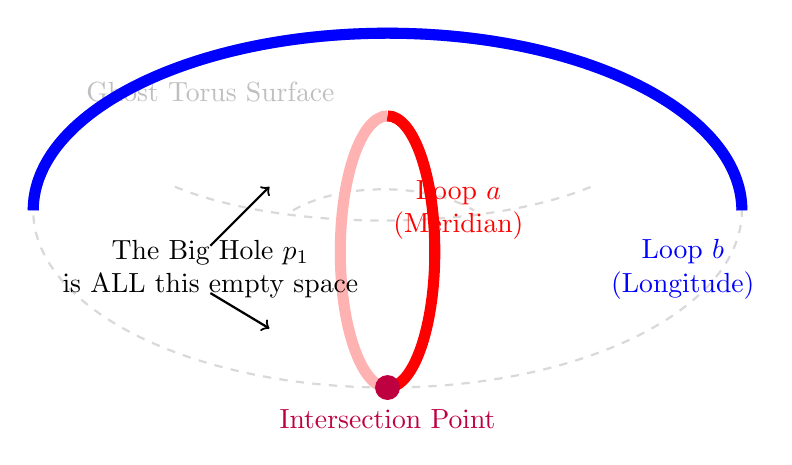
\begin{tikzpicture}[scale=1.5]
    % --- 1. 画幽灵环面 (Ghost Torus) ---
    % 用浅灰色虚线表示, 作为背景参考
    \draw[gray!30, dashed, thick] (0,0) ellipse (3cm and 1.5cm); % 外轮廓
    \draw[gray!30, dashed, thick] (-0.8,0) arc (140:40:1cm and 0.5cm); % 内圈上沿
    \draw[gray!30, dashed, thick] (-1.8,0.2) arc (220:320:2.3cm and 0.8cm); % 内圈下沿
    \node[gray!50] at (-1.5, 1) {Ghost Torus Surface};

    % --- 2. 画红色带子 (Meridian / 经线) ---
    % 这是一个竖直的圈, 绕着管子
    % 后半部分 (被挡住的, 画深一点颜色表示立体感)
    \draw[line width=4pt, red!30] (0, -1.5) arc (270:90:0.4cm and 1.15cm);
    
    % 前半部分
    \draw[line width=4pt, red] (0, 0.8) arc (90:-90:0.4cm and 1.15cm);
    
    % --- 3. 画蓝色带子 (Longitude / 纬线) ---
    % 这是一个水平的圈, 沿着长轴
    % 后半部分
    \draw[line width=4pt, blue!30] (-3,0) arc (180:0:3cm and 1.5cm);
    
    % 前半部分 (注意在交点处断开一下, 制造遮挡感, 或者直接画在上面)
    % 为了清晰, 我们让蓝色带子在交点处"穿过"红色带子
    \draw[line width=4pt, blue] (3,0) arc (0:180:3cm and 1.5cm);

    % --- 4. 强调交点 (Intersection) ---
    % 这是两个圈唯一的公共部分
    \fill[purple] (0, -1.5) circle (3pt);
    \node[purple, below] at (0, -1.6) {Intersection Point};

    % --- 5. 标注 ---
    \node[red, align=center] at (0.6, 0) {Loop $a$\\ (Meridian)};
    \node[blue, align=center] at (2.5, -0.5) {Loop $b$\\ (Longitude)};
    
    % 指出大洞在哪里
    \node[align=center] at (-1.5, -0.5) {The Big Hole $p_1$\\is ALL this empty space};
    \draw[->, thick, black] (-1.5, -0.3) -- (-1, 0.2);
    \draw[->, thick, black] (-1.5, -0.7) -- (-1, -1);

\end{tikzpicture}
\end{center}
不妨认为剩下两个点是在两个细纸带骨架上分别挖去一个的, 此时每个被挖去了一个点的纸带, 可以形变收缩到以交点为基点的 \(  S^{1}\vee S^{1}  \).   具体体现为以下过程
\begin{center}
  
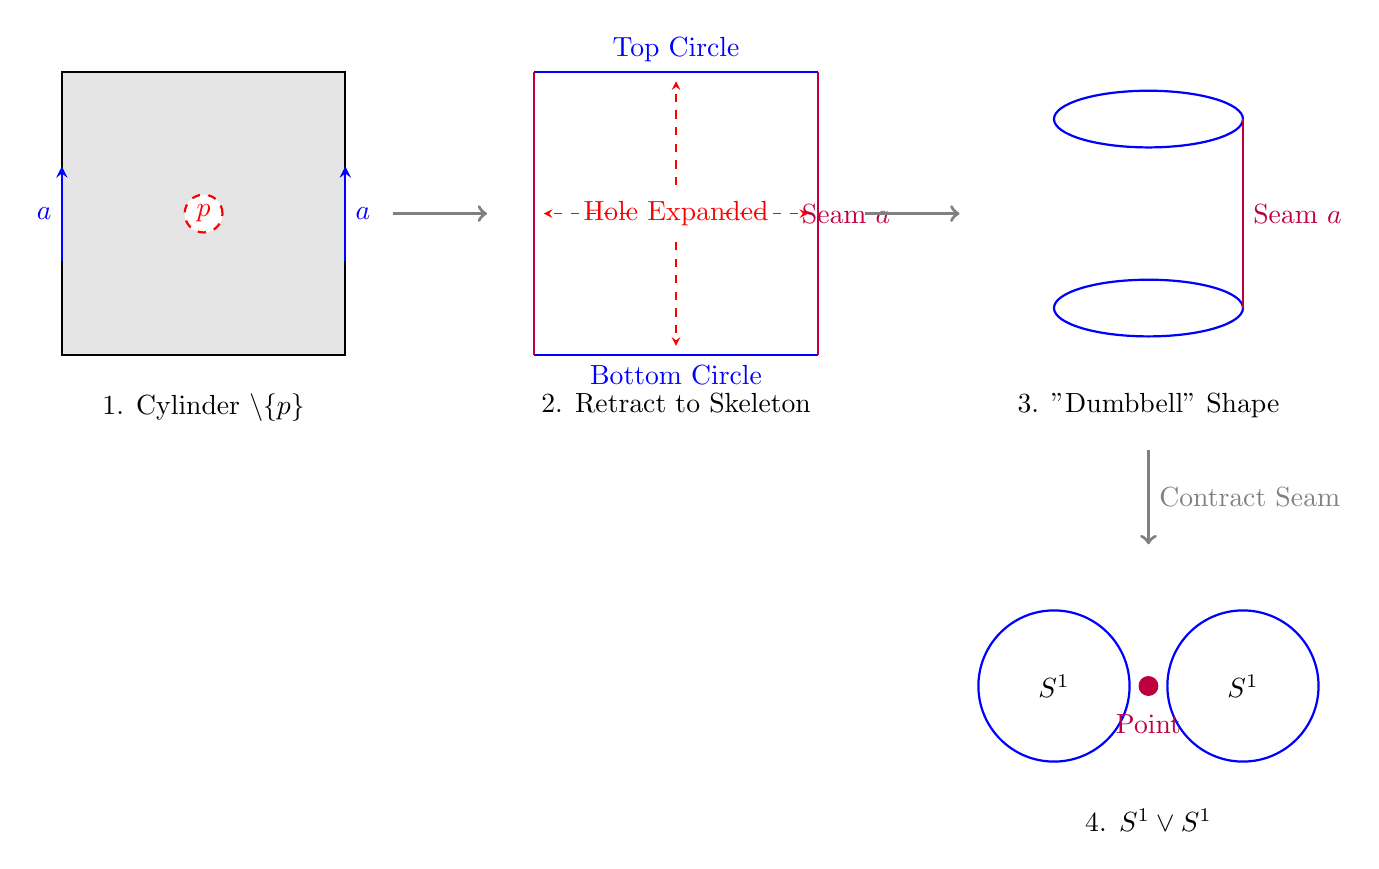
\begin{tikzpicture}[scale=1.2]
    % --- 样式定义 ---
    \tikzstyle{arrowstyle}=[->, >=stealth, thick, blue]
    \tikzstyle{force}=[->, >=stealth, red, dashed]

    % ====== 步骤 1: 纸带与挖洞 (The Cylinder with a Hole) ======
    \begin{scope}[shift={(0,0)}]
        % 矩形区域
        \fill[gray!20] (-1.5,-1.5) rectangle (1.5,1.5);
        \draw[thick] (-1.5,-1.5) rectangle (1.5,1.5);
        
        % 左右粘合标记
        \draw[arrowstyle] (-1.5, -0.5) -- (-1.5, 0.5) node[midway, left] {$a$};
        \draw[arrowstyle] (1.5, -0.5) -- (1.5, 0.5) node[midway, right] {$a$};
        
        % 挖掉的点
        \fill[white] (0,0) circle (0.2);
        \draw[red, thick, dashed] (0,0) circle (0.2);
        \node[red] at (0,0) {$p$};
        
        % 标题
        \node[below] at (0, -1.8) {1. Cylinder $\setminus \{p\}$};
    \end{scope}

    % 箭头指向下一步
    \draw[->, very thick, gray] (2, 0) -- (3, 0);

    % ====== 步骤 2: 洞膨胀/收缩到骨架 (Retraction) ======
    \begin{scope}[shift={(5,0)}]
        % 幽灵矩形
        \draw[gray!30, dashed] (-1.5,-1.5) rectangle (1.5,1.5);
        
        % 骨架 (Skeleton)
        % 上边界
        \draw[thick, blue] (-1.5, 1.5) -- (1.5, 1.5) node[midway, above] {Top Circle};
        % 下边界
        \draw[thick, blue] (-1.5, -1.5) -- (1.5, -1.5) node[midway, below] {Bottom Circle};
        % 粘合线 (因为左右粘合, 所以左右两条线其实是一条线)
        \draw[thick, purple] (-1.5, -1.5) -- (-1.5, 1.5);
        \draw[thick, purple] (1.5, -1.5) -- (1.5, 1.5);
        \node[purple] at (1.8, 0) {Seam $a$};
        
        % 力的示意
        \node[red] at (0,0) {Hole Expanded};
        \draw[force] (0,0.3) -- (0, 1.4);
        \draw[force] (0,-0.3) -- (0, -1.4);
        \draw[force] (0.5,0) -- (1.4, 0);
        \draw[force] (-0.5,0) -- (-1.4, 0);
        
        % 标题
        \node[below] at (0, -1.8) {2. Retract to Skeleton};
    \end{scope}

    % 箭头指向下一步
    \draw[->, very thick, gray] (7, 0) -- (8, 0);

    % ====== 步骤 3: 哑铃形/Theta图 (The Dumbbell) ======
    % 这是一个中间状态, 把上面的矩形左右粘起来看
    \begin{scope}[shift={(10,0)}]
        % 上圆
        \draw[thick, blue] (0, 1) ellipse (1cm and 0.3cm);
        % 下圆
        \draw[thick, blue] (0, -1) ellipse (1cm and 0.3cm);
        % 连接线 (Seam)
        \draw[thick, purple] (1, 1) -- (1, -1) node[midway, right] {Seam $a$};
        
        % 标题
        \node[below] at (0, -1.8) {3. "Dumbbell" Shape};
    \end{scope}
    
    % 箭头指向下一步 (同伦收缩)
    \draw[->, very thick, gray] (10, -2.5) -- (10, -3.5) node[midway, right] {Contract Seam};

    % ====== 步骤 4: 最终结果 (Wedge Sum) ======
    \begin{scope}[shift={(10,-5)}]
        % 左圆
        \draw[thick, blue] (-1, 0) circle (0.8);
        \node at (-1, 0) {$S^1$};
        
        % 右圆
        \draw[thick, blue] (1, 0) circle (0.8);
        \node at (1, 0) {$S^1$};
        
        % 粘合点
        \fill[purple] (0,0) circle (3pt);
        \node[purple, below] at (0, -0.2) {Point};
        
        % 标题
        \node[below] at (0, -1.2) {4. $S^1 \vee S^1$};
    \end{scope}

\end{tikzpicture}
\end{center}

故 \[
 \pi _1 \left( T^{2}\setminus \left\{ p_1,p_2,p_3 \right\} \right) \simeq  \pi _1 \left( S^{1}\vee S^{1}\vee  S^{1}\vee  S^{1} \right)\simeq \mathbb{Z} *\mathbb{Z} *\mathbb{Z} *\mathbb{Z}   
\]

\item 弧 \(  C  \)是可缩空间, 将其收缩为一点 \(  C\to \left\{ q \right\}  \)是同伦等价的变换. 收缩后 \(  p,q  \)重合, 弧 \(  A,B  \)成为以该点为基点的两个圈. 故 \[
 \pi _1 \left(  \theta  \right)\simeq  \pi _1 \left( S^{1}\vee S^{1} \right)\simeq \mathbb{Z} *\mathbb{Z}   
\]    
    \end{enumerate}
   
\end{proof}

\begin{exercise}{}{}
设 \(G_1,G_2,H\) 是 \(3\) 个群, \(f_i:G_i\to H\) 是同态 \(i=1,2\). 证明存在唯一同态 \(\varphi:G_1*G_2\to H\) 使得 \(\varphi|_{G_i}=f_i\).
\end{exercise}

\begin{proof}
   设\(  \iota _1 :G_1\to G_1*G_2  \)和 \(  \iota _2 :G_2\to G_1*G_2  \)是典范的单同态.  由于 \(  \iota_1 \left( G_1 \right)  \cup   \iota_2\left( G_2 \right)  \)生成了 \(  G_1*G_2  \), 我们有若 \(   \varphi _1 , \varphi _2   \)是群同态, 使得 \(   \varphi _1 \circ \iota _1 =  \varphi _2 \circ \iota _1 = f_1  \), \(   \varphi _1 \circ \iota _2 =  \varphi _2 \circ \iota _2  = f_2 \), 则 \(   \varphi _1 =  \varphi _2   \), 即满足条件的群同态若存在, 则是唯一的.
   
   
   对于 \(  G_1*G_2  \)中的既约字 \(  g_1\cdots g_{n}  \), 其中 \(  g_{i}\in G_{\alpha _{i}}, \alpha _{i}\in \left\{ 1,2 \right\}  \), 定义 \[
    \varphi \left( g_1\cdots g_{n} \right)= f_{\alpha _{1}}\left( g_1 \right)\cdots f_{\alpha _{n}}\left( g_{n} \right)   ,\quad  \varphi \left( e \right)= e_{H} 
   \]   
   且由于 \(  f_{i}  \)是群同态, 满足 \(  f_{i}\left( xy \right)= f_{i}\left( x \right)f_{i}\left( y \right)     \), \(  f_{i}\left( e \right)= e_{H}   \), 上述映射 \(   \varphi   \)与相邻字的合并和抵消操作交换, 故 \(   \varphi   \)是群同态.    
\end{proof}

\begin{exercise}{}{}
验证 Klein 瓶的基本群的两种表达式 \(\langle a,b\mid aba^{-1}b\rangle\) 和 \(\langle \alpha,\beta\mid \alpha^2\beta^2\rangle\) 是同构的.
\end{exercise}

\begin{proof}
    考虑群同态 \[
     \begin{aligned}
     \varphi : \left<\alpha , \beta  \right>&\to \left<a,b \right>\\ 
       \varphi \left( \alpha  \right)= a&,\quad  \varphi \left( \beta  \right)= a^{-1} b
     \end{aligned}
    \]并通过群同态的性质将定义扩张到 \(  \left<\alpha , \beta  \right>  \). 则 \(   \varphi   \)有逆同态 \[
    \begin{aligned}
    \psi  :\left<a,b \right>&\to \left<\alpha ,\beta  \right> \\ 
      \psi  \left( a \right)= \alpha ,&\quad  \psi \left( b \right)= \alpha \beta   
    \end{aligned}
    \]  注意到\[
     \varphi \left( \alpha ^{2}\beta ^{2} \right)= a^{2} a^{-1} ba^{-1} b= aba^{-1} b
    \] 这表明 \(   \varphi   \left( \left<\alpha ^{2}\beta ^{2} \right> \right)= \left<aba^{-1} b \right> \). 故 由商的泛性质, \(   \varphi   \)诱导出群同态 \(   \bar{\varphi}: \left<\alpha ,\beta  |\alpha ^{2}\beta ^{2}\right>\to \left<a,b|aba^{-1} b \right>  \). 类似地, 由 \(  \psi \left( aba^{-1} b \right)= \alpha ^{2}\beta ^{2}   \)     , 可知 \(  \psi   \)诱导出群同态 \(  \bar{\psi}: \left<a,b| aba^{-1} b \right>\to \left<\alpha ,\beta | \alpha ^{2}\beta ^{2} \right>  \). 直接验证可得 \(   \bar{\varphi}\circ \bar{\psi}= \operatorname{Id}  \), \(  \bar{\psi}\circ  \bar{\varphi}= \operatorname{Id}  \), 故 \(   \bar{\varphi}  \)是群同构. 因此 \(  \left<a,b|aba^{-1} b \right>  \)和 \(  \left<\alpha ,\beta | \alpha ^{2}\beta ^{2} \right>  \)同构.       
\end{proof}
\end{document}